% Options for packages loaded elsewhere
\PassOptionsToPackage{unicode}{hyperref}
\PassOptionsToPackage{hyphens}{url}
\PassOptionsToPackage{dvipsnames,svgnames,x11names}{xcolor}
%
\documentclass[
  letterpaper,
  DIV=11,
  numbers=noendperiod]{scrartcl}

\usepackage{amsmath,amssymb}
\usepackage{iftex}
\ifPDFTeX
  \usepackage[T1]{fontenc}
  \usepackage[utf8]{inputenc}
  \usepackage{textcomp} % provide euro and other symbols
\else % if luatex or xetex
  \usepackage{unicode-math}
  \defaultfontfeatures{Scale=MatchLowercase}
  \defaultfontfeatures[\rmfamily]{Ligatures=TeX,Scale=1}
\fi
\usepackage{lmodern}
\ifPDFTeX\else  
    % xetex/luatex font selection
\fi
% Use upquote if available, for straight quotes in verbatim environments
\IfFileExists{upquote.sty}{\usepackage{upquote}}{}
\IfFileExists{microtype.sty}{% use microtype if available
  \usepackage[]{microtype}
  \UseMicrotypeSet[protrusion]{basicmath} % disable protrusion for tt fonts
}{}
\makeatletter
\@ifundefined{KOMAClassName}{% if non-KOMA class
  \IfFileExists{parskip.sty}{%
    \usepackage{parskip}
  }{% else
    \setlength{\parindent}{0pt}
    \setlength{\parskip}{6pt plus 2pt minus 1pt}}
}{% if KOMA class
  \KOMAoptions{parskip=half}}
\makeatother
\usepackage{xcolor}
\setlength{\emergencystretch}{3em} % prevent overfull lines
\setcounter{secnumdepth}{-\maxdimen} % remove section numbering
% Make \paragraph and \subparagraph free-standing
\ifx\paragraph\undefined\else
  \let\oldparagraph\paragraph
  \renewcommand{\paragraph}[1]{\oldparagraph{#1}\mbox{}}
\fi
\ifx\subparagraph\undefined\else
  \let\oldsubparagraph\subparagraph
  \renewcommand{\subparagraph}[1]{\oldsubparagraph{#1}\mbox{}}
\fi


\providecommand{\tightlist}{%
  \setlength{\itemsep}{0pt}\setlength{\parskip}{0pt}}\usepackage{longtable,booktabs,array}
\usepackage{calc} % for calculating minipage widths
% Correct order of tables after \paragraph or \subparagraph
\usepackage{etoolbox}
\makeatletter
\patchcmd\longtable{\par}{\if@noskipsec\mbox{}\fi\par}{}{}
\makeatother
% Allow footnotes in longtable head/foot
\IfFileExists{footnotehyper.sty}{\usepackage{footnotehyper}}{\usepackage{footnote}}
\makesavenoteenv{longtable}
\usepackage{graphicx}
\makeatletter
\def\maxwidth{\ifdim\Gin@nat@width>\linewidth\linewidth\else\Gin@nat@width\fi}
\def\maxheight{\ifdim\Gin@nat@height>\textheight\textheight\else\Gin@nat@height\fi}
\makeatother
% Scale images if necessary, so that they will not overflow the page
% margins by default, and it is still possible to overwrite the defaults
% using explicit options in \includegraphics[width, height, ...]{}
\setkeys{Gin}{width=\maxwidth,height=\maxheight,keepaspectratio}
% Set default figure placement to htbp
\makeatletter
\def\fps@figure{htbp}
\makeatother

\usepackage{booktabs}
\usepackage{longtable}
\usepackage{array}
\usepackage{multirow}
\usepackage{wrapfig}
\usepackage{float}
\usepackage{colortbl}
\usepackage{pdflscape}
\usepackage{tabu}
\usepackage{threeparttable}
\usepackage{threeparttablex}
\usepackage[normalem]{ulem}
\usepackage{makecell}
\usepackage{xcolor}
\KOMAoption{captions}{tableheading}
\makeatletter
\makeatother
\makeatletter
\makeatother
\makeatletter
\@ifpackageloaded{caption}{}{\usepackage{caption}}
\AtBeginDocument{%
\ifdefined\contentsname
  \renewcommand*\contentsname{Table of contents}
\else
  \newcommand\contentsname{Table of contents}
\fi
\ifdefined\listfigurename
  \renewcommand*\listfigurename{List of Figures}
\else
  \newcommand\listfigurename{List of Figures}
\fi
\ifdefined\listtablename
  \renewcommand*\listtablename{List of Tables}
\else
  \newcommand\listtablename{List of Tables}
\fi
\ifdefined\figurename
  \renewcommand*\figurename{Figure}
\else
  \newcommand\figurename{Figure}
\fi
\ifdefined\tablename
  \renewcommand*\tablename{Table}
\else
  \newcommand\tablename{Table}
\fi
}
\@ifpackageloaded{float}{}{\usepackage{float}}
\floatstyle{ruled}
\@ifundefined{c@chapter}{\newfloat{codelisting}{h}{lop}}{\newfloat{codelisting}{h}{lop}[chapter]}
\floatname{codelisting}{Listing}
\newcommand*\listoflistings{\listof{codelisting}{List of Listings}}
\makeatother
\makeatletter
\@ifpackageloaded{caption}{}{\usepackage{caption}}
\@ifpackageloaded{subcaption}{}{\usepackage{subcaption}}
\makeatother
\makeatletter
\@ifpackageloaded{tcolorbox}{}{\usepackage[skins,breakable]{tcolorbox}}
\makeatother
\makeatletter
\@ifundefined{shadecolor}{\definecolor{shadecolor}{rgb}{.97, .97, .97}}
\makeatother
\makeatletter
\makeatother
\makeatletter
\makeatother
\makeatletter
\@ifpackageloaded{fontawesome5}{}{\usepackage{fontawesome5}}
\makeatother
\ifLuaTeX
  \usepackage{selnolig}  % disable illegal ligatures
\fi
\IfFileExists{bookmark.sty}{\usepackage{bookmark}}{\usepackage{hyperref}}
\IfFileExists{xurl.sty}{\usepackage{xurl}}{} % add URL line breaks if available
\urlstyle{same} % disable monospaced font for URLs
\hypersetup{
  colorlinks=true,
  linkcolor={blue},
  filecolor={Maroon},
  citecolor={Blue},
  urlcolor={Blue},
  pdfcreator={LaTeX via pandoc}}

\author{}
\date{}

\begin{document}
\ifdefined\Shaded\renewenvironment{Shaded}{\begin{tcolorbox}[sharp corners, frame hidden, interior hidden, enhanced, boxrule=0pt, breakable, borderline west={3pt}{0pt}{shadecolor}]}{\end{tcolorbox}}\fi

\hypertarget{keyword}{%
\subsection{}\label{keyword}}

What words or phrases do you think of when you hear the word
{``Harvard''}?

This being a {data} class, I'd like to collect some data related to
{``statistical thinking.''}

Go to \href{https://bit.ly/stat-100-think}{bit.ly/stat-100-think} to
provide the words or phrases you think of when you hear {``statistical
thinking.''}

\begin{center}\rule{0.5\linewidth}{0.5pt}\end{center}

\includegraphics[width=1\textwidth,height=\textheight]{img/DAW.png}

{Statistical Thinking}

{Kelly McConville}

{Stat 100 Week 1 \textbar{} Fall 2023}

\begin{center}\rule{0.5\linewidth}{0.5pt}\end{center}

\hypertarget{getting-started-in-stat-100}{%
\subsection{Getting Started in Stat
100}\label{getting-started-in-stat-100}}

\hypertarget{step-1-getting-started-module-in-canvas}{%
\paragraph{Step 1: Getting Started Module in
Canvas}\label{step-1-getting-started-module-in-canvas}}

\includegraphics[width=0.85\textwidth,height=\textheight]{img/Canvas_getting_started.png}

\begin{center}\rule{0.5\linewidth}{0.5pt}\end{center}

\hypertarget{stat-100-tech-materials}{%
\subsection{Stat 100 Tech \& Materials}\label{stat-100-tech-materials}}

\includegraphics[width=0.65\textwidth,height=\textheight]{img/structures.001.jpeg}

\begin{center}\rule{0.5\linewidth}{0.5pt}\end{center}

\hypertarget{announcements}{%
\subsection{Announcements}\label{announcements}}

\begin{itemize}
\item
  Lecture slide decks will always be posted and linked to a Canvas
  Module the day before lecture.

  \begin{itemize}
  \tightlist
  \item
    Will also bring printed versions for those who prefer paper copies.
  \end{itemize}
\item
  No section and no lecture quiz this week.

  \begin{itemize}
  \tightlist
  \item
    But be on the look-out for section preference form from my.harvard.
  \end{itemize}
\item
  Only I will be running office hours this week at the following time:

  \begin{itemize}
  \tightlist
  \item
    Today 1:30 - 3:00 pm in Science Center 316 (This week only)
  \end{itemize}
\item
  The regular office hour schedule will be posted later this week and
  will start next week.
\item
  \textbf{If able, please bring a laptop or tablet to Mondays's
  lecture.}
\end{itemize}

\begin{center}\rule{0.5\linewidth}{0.5pt}\end{center}

\hypertarget{day-1-goals}{%
\subsection{Day 1 Goals}\label{day-1-goals}}

\begin{itemize}
\item
  Start engaging in statistical thinking
\item
  Introduce data
\item
  Consider hand-drawn visualizations as a way to tell stories with data
\item
  Hop into the RStudio Server using Posit Cloud
\end{itemize}

\begin{center}\rule{0.5\linewidth}{0.5pt}\end{center}

\hypertarget{looking-ahead-to-day-2}{%
\subsection{Looking Ahead to Day
2\ldots{}}\label{looking-ahead-to-day-2}}

\begin{itemize}
\item
  Discuss course structure (lecture, section, wrap-ups, office hours,
  assessments\ldots)
\item
  Present important course policies (engagement, code of conduct,
  chatGPT, \ldots)
\item
  Get started in \texttt{RStudio} and with \texttt{Quarto} documents
\end{itemize}

\hypertarget{but-first-let-me-quickly-introduce-myself}{%
\section{But first, let me quickly introduce
myself\ldots{}}\label{but-first-let-me-quickly-introduce-myself}}

\begin{center}\rule{0.5\linewidth}{0.5pt}\end{center}

\hypertarget{lets-start-with-my-path-to-harvard}{%
\subsubsection{Let's start with my path to
Harvard\ldots{}}\label{lets-start-with-my-path-to-harvard}}

\begin{figure}

{\centering \includegraphics[width=0.8\textwidth,height=\textheight]{stat100_wk01wed_files/figure-pdf/unnamed-chunk-2-1.pdf}

}

\end{figure}

\begin{center}\rule{0.5\linewidth}{0.5pt}\end{center}

\hypertarget{research-interests}{%
\subsection{Research Interests}\label{research-interests}}

\hypertarget{survey-statistics-and-collaborate-with}{%
\subsubsection{Survey statistics and collaborate
with}\label{survey-statistics-and-collaborate-with}}

\includegraphics[width=0.6\textwidth,height=\textheight]{img/logos.jpeg}

\begin{center}\rule{0.5\linewidth}{0.5pt}\end{center}

\hypertarget{research-interests-1}{%
\subsection{Research Interests}\label{research-interests-1}}

\hypertarget{where-survey-statistics-meets-data-science}{%
\subsubsection{Where survey statistics meets data
science}\label{where-survey-statistics-meets-data-science}}

\begin{figure}

{\centering \includegraphics[width=3.53in,height=\textheight]{img/data.jpeg}

}

\end{figure}

\begin{center}\rule{0.5\linewidth}{0.5pt}\end{center}

\hypertarget{advising-undergraduate-forestry-data-science-research}{%
\subsubsection{Advising Undergraduate Forestry Data Science
Research}\label{advising-undergraduate-forestry-data-science-research}}

\begin{figure}

\begin{minipage}[t]{0.50\linewidth}

{\centering 

\raisebox{-\height}{

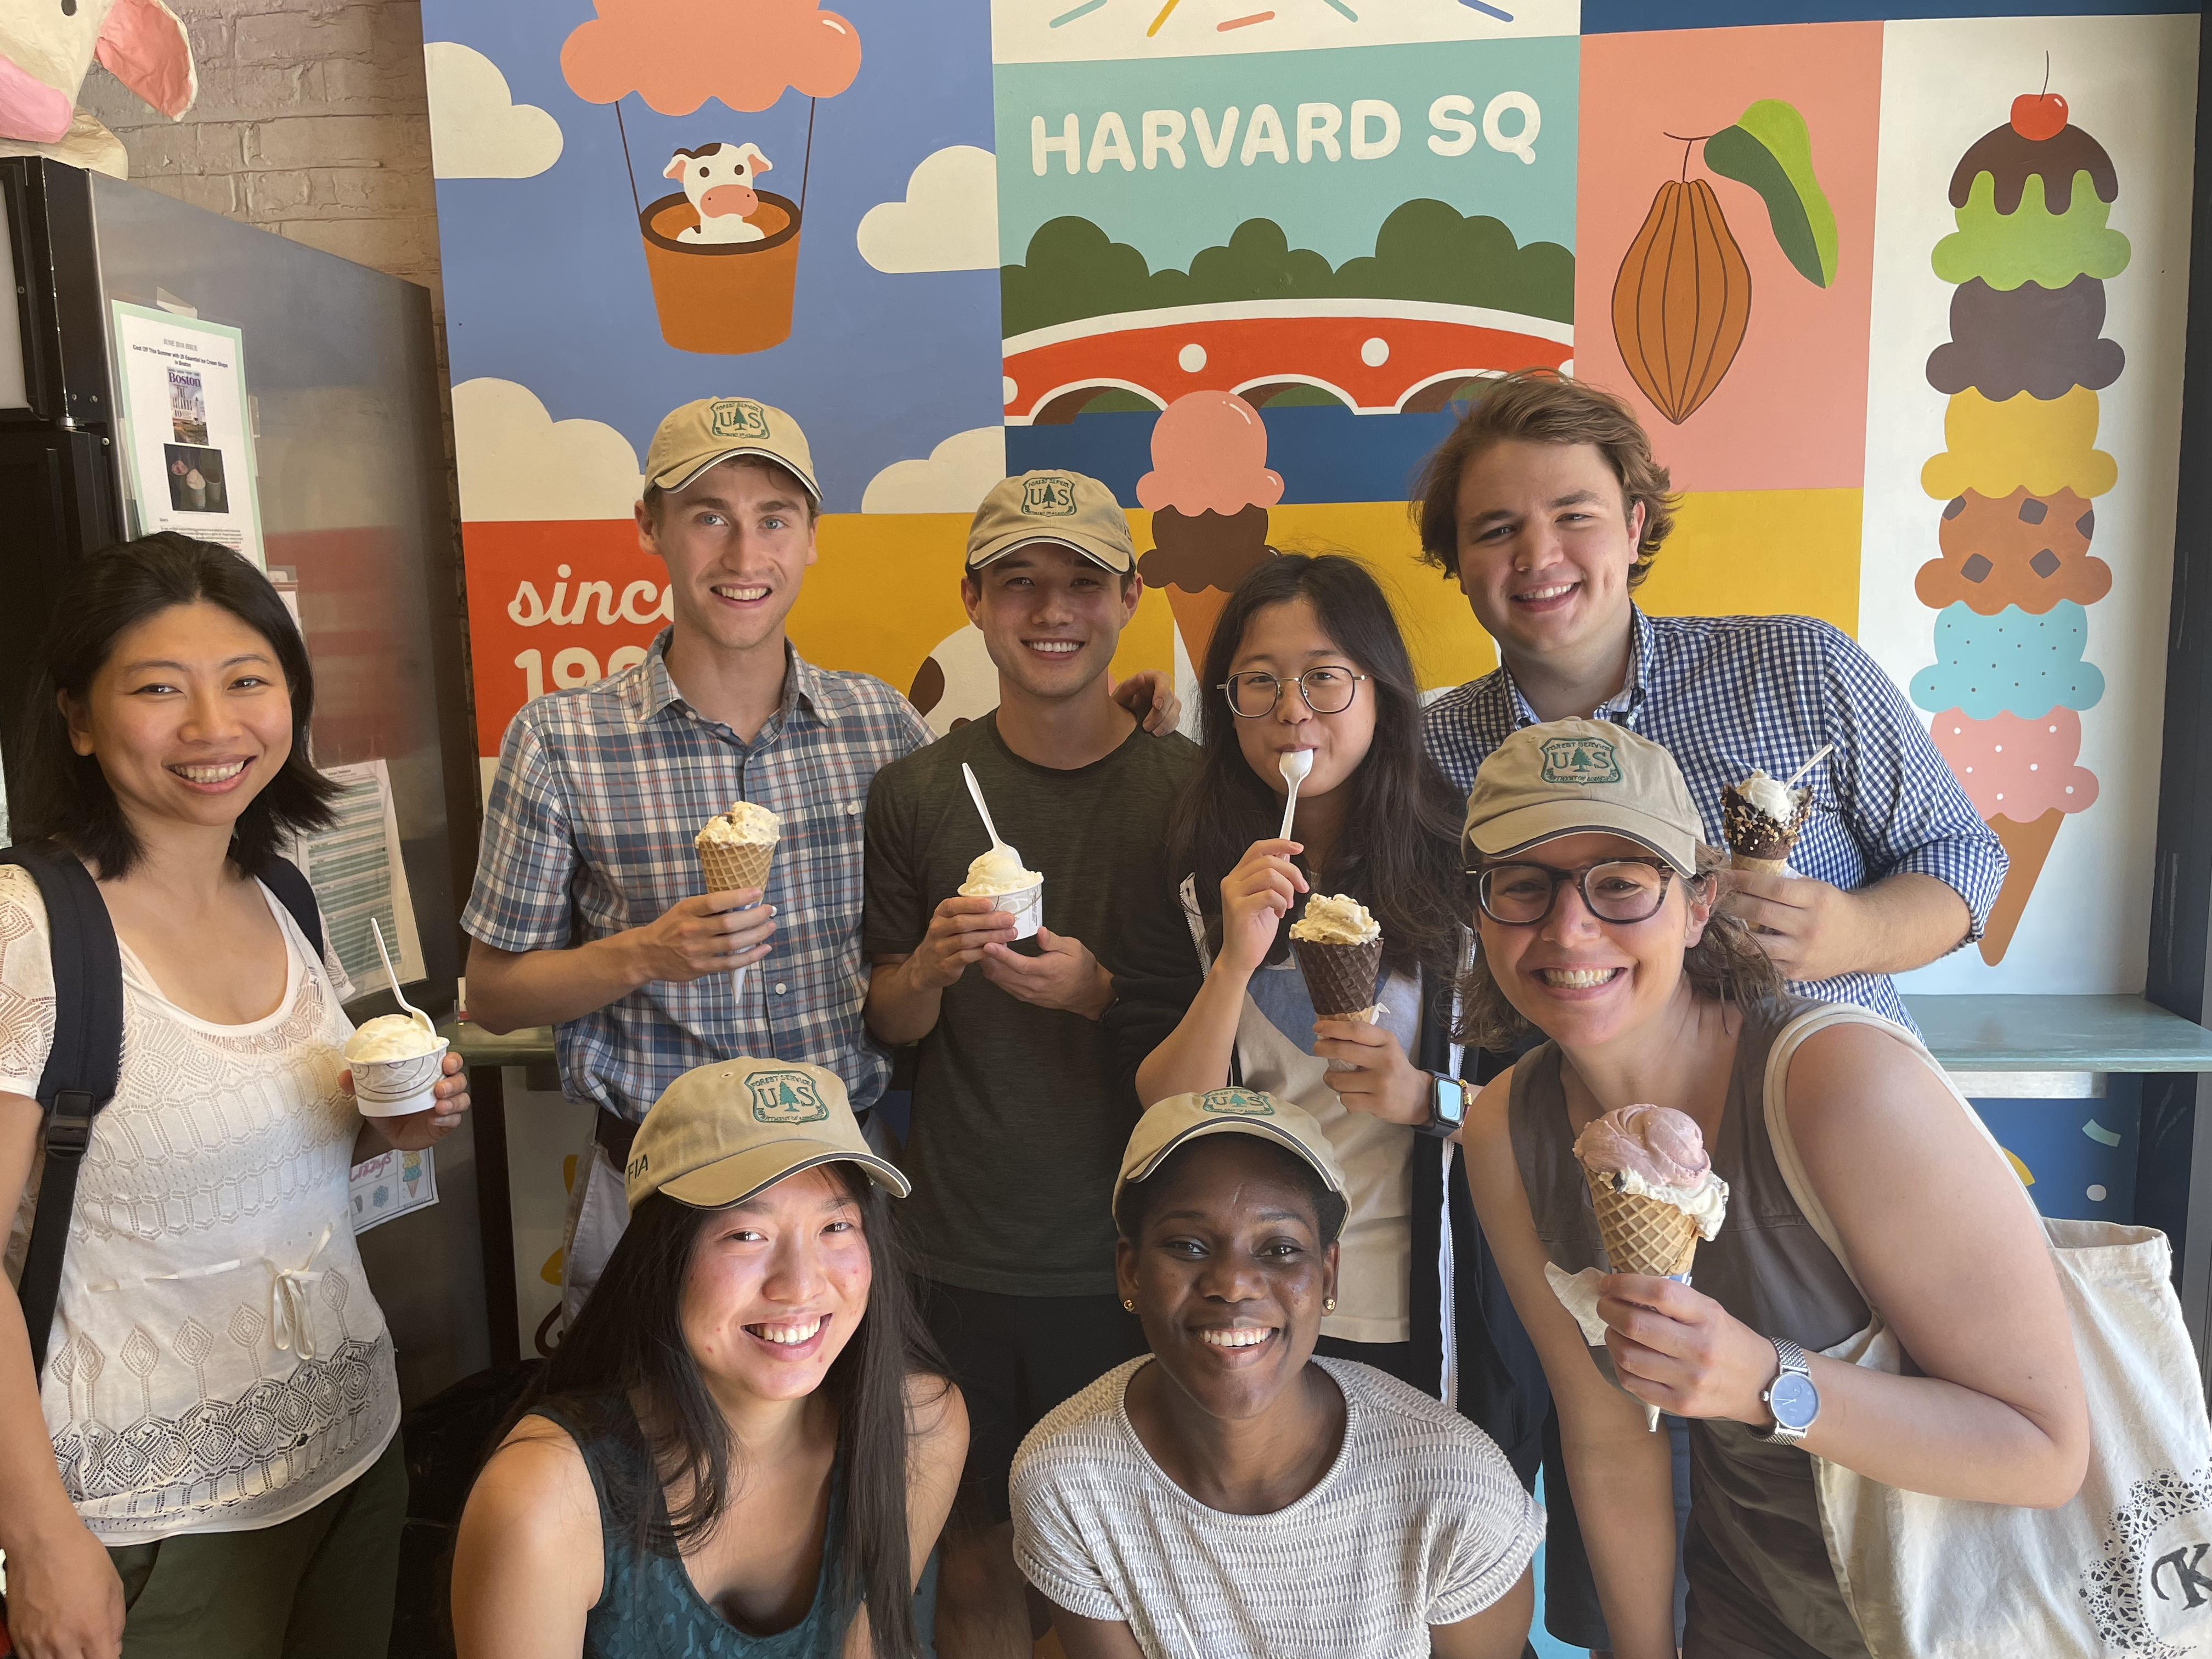
\includegraphics{img/Forest_and_IceCream_Lovers.jpg}

}

}

\end{minipage}%
%
\begin{minipage}[t]{0.50\linewidth}

{\centering 

\raisebox{-\height}{

\includegraphics{img/ufds_icecream_2023.jpg}

}

}

\end{minipage}%

\end{figure}

\begin{center}\rule{0.5\linewidth}{0.5pt}\end{center}

\includegraphics[width=0.8\textwidth,height=\textheight]{img/seedlings.jpg}

\hfill\break
\hfill\break

\begin{itemize}
\tightlist
\item
  I \textbf{love} teaching stats and coding.
\end{itemize}

\hfill\break

\begin{itemize}
\tightlist
\item
  But, learning stats and coding is \textbf{hard}.
\end{itemize}

\hfill\break

\begin{itemize}
\tightlist
\item
  With the \textbf{right scaffolding}, \textbf{good strategies}, and
  \textbf{sustained effort}, you can excel at both!
\end{itemize}

\hfill\break

\begin{itemize}
\tightlist
\item
  And mistakes are part of the learning process. They don't imply that
  you are bad at stats.
\end{itemize}

\hypertarget{also-the-stat-100-teaching-team-are-so-excited-to-support-your-learning}{%
\section{Also, the Stat 100 Teaching Team are so excited to support your
learning!}\label{also-the-stat-100-teaching-team-are-so-excited-to-support-your-learning}}

\begin{center}\rule{0.5\linewidth}{0.5pt}\end{center}

\hypertarget{stat-100-is-about-developing-our-statistical-thinking-skills.}{%
\subsection{\texorpdfstring{Stat 100 is about developing our
\textbf{statistical thinking}
skills.}{Stat 100 is about developing our statistical thinking skills.}}\label{stat-100-is-about-developing-our-statistical-thinking-skills.}}

What is \textbf{statistical thinking}?

It is not the same as mathematical thinking.

Let's discover what \textbf{statistical thinking} is through some
examples.

\begin{center}\rule{0.5\linewidth}{0.5pt}\end{center}

\hypertarget{data-in-stat-100}{%
\subsection{Data in Stat 100}\label{data-in-stat-100}}

Will use a wide-range of \textbf{real} and \textbf{relevant} data
examples

\includegraphics[width=1\textwidth,height=\textheight]{img/bls_ce_graph.png}

\includegraphics[width=0.8\textwidth,height=\textheight]{img/cambridge_trees.png}

\begin{center}\rule{0.5\linewidth}{0.5pt}\end{center}

\hypertarget{data-in-stat-100-1}{%
\subsection{Data in Stat 100}\label{data-in-stat-100-1}}

\includegraphics[width=1\textwidth,height=\textheight]{img/nytimes_opp_insights.png}

\includegraphics[width=0.8\textwidth,height=\textheight]{img/kate_petrova_candles.jpg}

\begin{itemize}
\item
  I understand that some of these topics have likely had profound
  impacts on your lives.
\item
  We will focus class time on the key course objectives but will use
  these current topics to empower ourselves and to see how we can
  productively participate with data.
\end{itemize}

\hypertarget{example-visualizing-covid-prevalence}{%
\section{Example: Visualizing COVID
Prevalence}\label{example-visualizing-covid-prevalence}}

\begin{center}\rule{0.5\linewidth}{0.5pt}\end{center}

\hypertarget{example-visualizing-covid-prevalence-1}{%
\subsubsection{Example: Visualizing COVID
Prevalence}\label{example-visualizing-covid-prevalence-1}}

\begin{itemize}
\tightlist
\item
  In May of 2020, the Georgia Department of Public Health posted the
  following graph:
\end{itemize}

\begin{figure}

{\centering \includegraphics[width=0.5\textwidth,height=\textheight]{img/GAcovid.jpg}

}

\end{figure}

\begin{itemize}
\item
  At a quick first glance, what story does the Georgia Department of
  Public Health graph appear to be telling?
\item
  What is misleading about the Georgia Department of Public Health
  graph? How could we fix this issue?
\end{itemize}

\begin{center}\rule{0.5\linewidth}{0.5pt}\end{center}

\hypertarget{example-visualizing-covid-prevalence-2}{%
\subsubsection{Example: Visualizing COVID
Prevalence}\label{example-visualizing-covid-prevalence-2}}

\begin{itemize}
\tightlist
\item
  After public outcry, the Georgia Department of Public Health said they
  made a mistake and posted the following updated graph:
\end{itemize}

\begin{figure}

{\centering \includegraphics[width=0.5\textwidth,height=\textheight]{img/GAcovid2.jpg}

}

\end{figure}

\begin{itemize}
\tightlist
\item
  How do your conclusions about COVID-19 cases in Georgia change when
  now interpreting this new graph?
\end{itemize}

\begin{center}\rule{0.5\linewidth}{0.5pt}\end{center}

Alberto Cairo, a journalist and designer, created the second graph of
the Georgia COVID-19 data:

\includegraphics[width=0.4\textwidth,height=\textheight]{img/GAcovid2.jpg}
\includegraphics[width=0.4\textwidth,height=\textheight]{img/GAcovid_cairo.png}

\begin{itemize}
\item
  A key principle of data visualization is to \textbf{``help the viewer
  make meaningful comparisons''}.
\item
  What comparisons are made easy by the lefthand graph? What about by
  the righthand graph?
\item
  From these graphs, can we get an accurate estimate of the COVID
  prevalence in these Georgian counties over this two week period?
\end{itemize}

\begin{center}\rule{0.5\linewidth}{0.5pt}\end{center}

\hypertarget{example-visualizing-covid-prevalence-3}{%
\subsubsection{Example: Visualizing COVID
Prevalence}\label{example-visualizing-covid-prevalence-3}}

\begin{itemize}
\tightlist
\item
  The \href{https://www.mwra.com/biobot/biobotdata.htm}{Massachusetts
  Water Resources Authority (MWRA) graph} tracks the presence of
  COVID-19 in the Boston-area wastewater.
\end{itemize}

\begin{figure}

{\centering \includegraphics[width=28.125in,height=\textheight]{stat100_wk01wed_files/figure-pdf/unnamed-chunk-4-1.pdf}

}

\end{figure}

\begin{itemize}
\item
  What are the pros of using wastewater over nasal swabs to assess COVID
  prevalence? What are the cons?
\item
  One more note: The graph also incorporates \textbf{uncertainty
  measures}, a key statistical thinking idea that we will learn more
  about later in the semester!
\end{itemize}

\begin{center}\rule{0.5\linewidth}{0.5pt}\end{center}

\hypertarget{what-is-statistical-thinking}{%
\section{What is ``Statistical
Thinking?''}\label{what-is-statistical-thinking}}

\begin{center}\rule{0.5\linewidth}{0.5pt}\end{center}

\hypertarget{statistical-thinking}{%
\subsection{Statistical Thinking}\label{statistical-thinking}}

\begin{itemize}
\tightlist
\item
  Understanding the importance of \textbf{context}.
\end{itemize}

\faIcon{arrow-right} Context explains the Monday jumps in the COVID
counts.

\begin{itemize}
\tightlist
\item
  How we \textbf{encode} information in a graph should be driven by our
  research question.
\end{itemize}

\faIcon{arrow-right} \textbf{Design choices} impact the conclusions the
viewer draws.

\begin{itemize}
\tightlist
\item
  How the data are \textbf{collected} impacts the conclusions we can
  draw.
\end{itemize}

\faIcon{arrow-right} Voluntary COVID test results don't likely provide
good estimates of COVID prevalence.

\begin{itemize}
\tightlist
\item
  Often we are using a \textbf{sample} of data to say something about a
  larger group. In this case, we should measure how certain our
  estimates are!
\end{itemize}

\faIcon{arrow-right} We will learn to \textbf{compute} and
\textbf{interpret} certainty estimates (like those in the wastewater
graph) later in the course!

\begin{center}\rule{0.5\linewidth}{0.5pt}\end{center}

\hypertarget{statistical-thinking-1}{%
\subsection{Statistical Thinking}\label{statistical-thinking-1}}

\begin{itemize}
\item
  About developing \textbf{reasoning} (not just learning definitions and
  formulae).
\item
  Developing our statistical thinking skills will allow us to soundly
  \textbf{extract knowledge from data}!
\item
  Statistical thinking requires \textbf{judgment} that takes time to
  develop.

  \begin{itemize}
  \tightlist
  \item
    Will see \textbf{examples} and \textbf{practice} applying
    statistical thinking throughout the course.
  \end{itemize}
\end{itemize}

\begin{center}\rule{0.5\linewidth}{0.5pt}\end{center}

\hypertarget{what-areis-data}{%
\subsection{\texorpdfstring{{What are/is
Data?}}{What are/is Data?}}\label{what-areis-data}}

\emph{``\,`Raw data' is an oxymoron.''} -- Lisa Gitelman

\emph{``Data \ldots{} is information made tractable.''} -- Catherine
D'Ignazio and Lauren Klein

\begin{center}\rule{0.5\linewidth}{0.5pt}\end{center}

\hypertarget{data-frames}{%
\subsection{Data Frames}\label{data-frames}}

Data in \textbf{spreadsheet}-like format where:

\begin{itemize}
\item
  Rows = Observations/cases
\item
  Columns = Variables
\end{itemize}

\begin{table}
\centering\begingroup\fontsize{32}{34}\selectfont

\begin{tabular}{r|l|r|l|l|l|l|l}
\hline
ID & kind & .pred\_AI & .pred\_class & detector & native & name & model\\
\hline
1 & Human & 0.9999942 & AI & Sapling & No & Real TOEFL & Human\\
\hline
2 & Human & 0.8281448 & AI & Crossplag & No & Real TOEFL & Human\\
\hline
3 & Human & 0.0002137 & Human & Crossplag & Yes & Real College Essays & Human\\
\hline
4 & AI & 0.0000000 & Human & ZeroGPT & NA & Fake CS224N - GPT3 & GPT3\\
\hline
5 & AI & 0.0017841 & Human & OriginalityAI & NA & Fake CS224N - GPT3, PE & GPT4\\
\hline
6 & Human & 0.0001783 & Human & HFOpenAI & Yes & Real CS224N & Human\\
\hline
\end{tabular}
\endgroup{}
\end{table}

\begin{itemize}
\tightlist
\item
  Data from \textbf{GPT Detectors Are Biased Against Non-Native English
  Writers.} \emph{Weixin Liang}, \emph{Mert Yuksekgonul}, \emph{Yining
  Mao}, \emph{Eric Wu}, \emph{James Zou.}
  \href{https://doi.org/10.1016/j.patter.2023.100779}{CellPress
  Patterns} and available in the \texttt{R} package \texttt{detectors}.
\end{itemize}

\begin{center}\rule{0.5\linewidth}{0.5pt}\end{center}

\hypertarget{data-frames-1}{%
\subsection{Data Frames}\label{data-frames-1}}

\begin{table}
\centering\begingroup\fontsize{32}{34}\selectfont

\begin{tabular}{r|l|r|l|l|l|l|l}
\hline
ID & kind & .pred\_AI & .pred\_class & detector & native & name & model\\
\hline
1 & Human & 0.9999942 & AI & Sapling & No & Real TOEFL & Human\\
\hline
2 & Human & 0.8281448 & AI & Crossplag & No & Real TOEFL & Human\\
\hline
3 & Human & 0.0002137 & Human & Crossplag & Yes & Real College Essays & Human\\
\hline
4 & AI & 0.0000000 & Human & ZeroGPT & NA & Fake CS224N - GPT3 & GPT3\\
\hline
5 & AI & 0.0017841 & Human & OriginalityAI & NA & Fake CS224N - GPT3, PE & GPT4\\
\hline
6 & Human & 0.0001783 & Human & HFOpenAI & Yes & Real CS224N & Human\\
\hline
\end{tabular}
\endgroup{}
\end{table}

Rows = Observations/cases

\textbf{What are the cases? What does each row represent?}

\begin{center}\rule{0.5\linewidth}{0.5pt}\end{center}

\hypertarget{data-frames-2}{%
\subsection{Data Frames}\label{data-frames-2}}

\begin{table}
\centering\begingroup\fontsize{32}{34}\selectfont

\begin{tabular}{r|l|r|l|l|l|l|l}
\hline
ID & kind & .pred\_AI & .pred\_class & detector & native & name & model\\
\hline
1 & Human & 0.9999942 & AI & Sapling & No & Real TOEFL & Human\\
\hline
2 & Human & 0.8281448 & AI & Crossplag & No & Real TOEFL & Human\\
\hline
3 & Human & 0.0002137 & Human & Crossplag & Yes & Real College Essays & Human\\
\hline
4 & AI & 0.0000000 & Human & ZeroGPT & NA & Fake CS224N - GPT3 & GPT3\\
\hline
5 & AI & 0.0017841 & Human & OriginalityAI & NA & Fake CS224N - GPT3, PE & GPT4\\
\hline
6 & Human & 0.0001783 & Human & HFOpenAI & Yes & Real CS224N & Human\\
\hline
\end{tabular}
\endgroup{}
\end{table}

Columns = Variables

\textbf{Variables}: Describe characteristics of the observations

\begin{itemize}
\item
  \textbf{Quantitative}: Numerical in nature
\item
  \textbf{Categorical}: Values are categories
\item
  \textbf{Identification}: Uniquely identify each case
\end{itemize}

\begin{center}\rule{0.5\linewidth}{0.5pt}\end{center}

\begin{table}
\centering\begingroup\fontsize{32}{34}\selectfont

\begin{tabular}{r|l|r|l|l|l|l|l}
\hline
ID & kind & .pred\_AI & .pred\_class & detector & native & name & model\\
\hline
1 & Human & 0.9999942 & AI & Sapling & No & Real TOEFL & Human\\
\hline
2 & Human & 0.8281448 & AI & Crossplag & No & Real TOEFL & Human\\
\hline
3 & Human & 0.0002137 & Human & Crossplag & Yes & Real College Essays & Human\\
\hline
4 & AI & 0.0000000 & Human & ZeroGPT & NA & Fake CS224N - GPT3 & GPT3\\
\hline
5 & AI & 0.0017841 & Human & OriginalityAI & NA & Fake CS224N - GPT3, PE & GPT4\\
\hline
6 & Human & 0.0001783 & Human & HFOpenAI & Yes & Real CS224N & Human\\
\hline
\end{tabular}
\endgroup{}
\end{table}

Every time you get a new dataset, spend time exploring the variables.

Example questions:

\begin{itemize}
\item
  Is the variable capturing what I want?
\item
  For categorical variables, what are the categories? Do those
  categories adequately represent the data represented by that variable?
\item
  For quantitative variables, what values are possible? Were the data
  rounded or binned? Are those values actually encoding categories? What
  are the units of measurement?
\end{itemize}

\hypertarget{goal-start-collecting-data-from-your-life-so-that-you-can-visualize-it-on-p-set-1.}{%
\section{Goal: Start collecting data from your life so that you can
visualize it on P-Set
1.}\label{goal-start-collecting-data-from-your-life-so-that-you-can-visualize-it-on-p-set-1.}}

\begin{center}\rule{0.5\linewidth}{0.5pt}\end{center}

\hypertarget{hand-drawn-data-viz}{%
\subsection{Hand-Drawn Data Viz}\label{hand-drawn-data-viz}}

\begin{itemize}
\item
  Once we have collected data, a common next step is to visualize it.
\item
  Two key aspects of data visualization:

  \begin{itemize}
  \item
    Determining how you want to display the data.
  \item
    Figuring out how to tell the computer to do that mapping.
  \end{itemize}
\item
  Hand-drawn data visualizations allow us to focus on the first part
  with full control over the \textbf{creative} process!
\end{itemize}

\begin{center}\rule{0.5\linewidth}{0.5pt}\end{center}

\hypertarget{hand-drawn-data-viz-examples}{%
\subsection{Hand-Drawn Data Viz
Examples}\label{hand-drawn-data-viz-examples}}

\href{http://www.dear-data.com/theproject}{Dear Data}

\emph{``Each week, and for a year, we collected and measured a
particular type of data about our lives, used this data to make a
drawing on a postcard-sized sheet of paper, and then dropped the
postcard in an English''postbox'' (Stefanie) or an American ``mailbox''
(Giorgia)!{}``}

\begin{center}\rule{0.5\linewidth}{0.5pt}\end{center}

\hypertarget{dear-data-examples}{%
\subsubsection{Dear Data Examples}\label{dear-data-examples}}

\begin{figure}

{\centering \includegraphics[width=1\textwidth,height=\textheight]{img/complaints.png}

}

\end{figure}

\begin{center}\rule{0.5\linewidth}{0.5pt}\end{center}

\hypertarget{dear-data-examples-1}{%
\subsubsection{Dear Data Examples}\label{dear-data-examples-1}}

\begin{figure}

{\centering \includegraphics[width=1\textwidth,height=\textheight]{img/time.png}

}

\end{figure}

\begin{center}\rule{0.5\linewidth}{0.5pt}\end{center}

\hypertarget{more-dear-data-examples}{%
\subsubsection{More Dear Data Examples}\label{more-dear-data-examples}}

\begin{itemize}
\tightlist
\item
  Becky Cooper handed out hand-drawn maps of Manhattan to strangers and
  asked them to
  \href{https://www.goodreads.com/book/show/15842664-mapping-manhattan?from_search=true}{``map
  their Manhattan.''}
\end{itemize}

\begin{figure}

{\centering \includegraphics[width=0.8\textwidth,height=\textheight]{img/mapmanhattan.png}

}

\caption{Map drawn by New Yorker staff writer Patricia Marx}

\end{figure}

\begin{itemize}
\tightlist
\item
  What would the data frame for this visualization look like?
\end{itemize}

\begin{center}\rule{0.5\linewidth}{0.5pt}\end{center}

\hypertarget{more-dear-data-examples-1}{%
\subsubsection{More Dear Data
Examples}\label{more-dear-data-examples-1}}

\begin{figure}

{\centering \includegraphics[width=0.9\textwidth,height=\textheight]{img/postcards_stat100s22.001.jpeg}

}

\end{figure}

\begin{itemize}
\tightlist
\item
  What would the data frame for this visualization look like?
\end{itemize}

\begin{center}\rule{0.5\linewidth}{0.5pt}\end{center}

\hypertarget{more-dear-data-examples-2}{%
\subsubsection{More Dear Data
Examples}\label{more-dear-data-examples-2}}

\begin{figure}

{\centering \includegraphics[width=0.8\textwidth,height=\textheight]{img/postcards_stat100s22.002.jpeg}

}

\end{figure}

\begin{itemize}
\tightlist
\item
  What would the data frame for this visualization look like?
\end{itemize}

\begin{center}\rule{0.5\linewidth}{0.5pt}\end{center}

\hypertarget{goal-by-next-wed-collect-data-from-your-life-so-that-you-can-visualize-it-on-p-set-1.}{%
\subsection{Goal: By next Wed, collect data from your life so that you
can visualize it on P-Set
1.}\label{goal-by-next-wed-collect-data-from-your-life-so-that-you-can-visualize-it-on-p-set-1.}}

\hypertarget{recommendations}{%
\paragraph{Recommendations}\label{recommendations}}

\begin{itemize}
\item
  Store the data in your favorite spreadsheet program (Google Sheets,
  Numbers, Excel).
\item
  Determine what your cases/observations will be.
\item
  Collect data on \textbf{more} variables than you will likely
  visualize. It is hard to know beforehand what the interesting
  relationships will be.
\end{itemize}

\hypertarget{next-week}{%
\paragraph{Next Week}\label{next-week}}

\begin{itemize}
\tightlist
\item
  Will get a blank postcard and further guidance on the visualization
  with P-Set 1.
\end{itemize}

\begin{center}\rule{0.5\linewidth}{0.5pt}\end{center}

\hypertarget{section}{%
\subsection{}\label{section}}

Demo of accessing the RStudio Server on Posit Cloud

Try to access the RStudio Server between now and next lecture.

Come back to the recording if need help with the steps.

\begin{center}\rule{0.5\linewidth}{0.5pt}\end{center}

\begin{center}\rule{0.5\linewidth}{0.5pt}\end{center}

\hypertarget{reminders}{%
\subsection{Reminders}\label{reminders}}

\begin{itemize}
\item
  \textbf{If able, please bring a laptop or tablet to Mondays's
  lecture.}
\item
  No section, no wrap-ups, and no lecture quiz this week.
\item
  Make sure to go through the syllabus, which can be found on Canvas.

  \begin{itemize}
  \tightlist
  \item
    Will discuss assessments and course policies on Monday.
  \end{itemize}
\item
  Only I will be running office hours this week at the following time:

  \begin{itemize}
  \tightlist
  \item
    Today 1:30 - 3:00 pm in Science Center 316 (This week only)
  \end{itemize}
\item
  The regular office hour schedule will be posted later this week and
  will start next week.
\item
  Be on the look-out for the section preference form.
\end{itemize}



\end{document}
